\documentclass[aspectratio=169]{beamer}
\usetheme{Madrid}
\usecolortheme{default}

\usepackage[utf8]{inputenc}
\usepackage[T1]{fontenc}
\usepackage{booktabs}
\usepackage{amsmath}

\title[DDPG Stock Trading Reproduction]{Reproducing a DDPG-Based Stock Trading Strategy}
\author[Kontorousis, Meliani]{Yassine Meliani \and George Kontorousis}
\institute[]{McGill University}
\date{\today}

\begin{document}

\begin{frame}
  \titlepage
\end{frame}

\begin{frame}{1) Problem and Goal}
  \textbf{Problem:} Daily stock trading is a noisy sequential decision-making task.\\[0.5em]

  \textbf{Project objective:}
  \begin{itemize}
    \item Reproduce Liu et al. (2018) DDPG stock-trading setup.
    \item Use the same Dow Jones split and compare against:
      \begin{itemize}
        \item DJIA benchmark
        \item Min-variance portfolio baseline
      \end{itemize}
    \item Test whether TD3 improves stability and performance over DDPG.
  \end{itemize}

  \vspace{0.5em}
  % \textit{Speaker timing: ~35 seconds}
\end{frame}

\begin{frame}{2) Environment and MDP}
  \textbf{State:}
  \[
    s_t = [b_t,\; p_t^{(1..28)},\; h_t^{(1..28)}]
  \]
  where $b_t$ is cash, $p_t$ are prices, and $h_t$ are holdings.

  \vspace{0.5em}
  \textbf{Action:} integer trades per stock
  \[
    a_t = [a_t^{(1)}, \ldots, a_t^{(28)}],
    \qquad
    a_t^{(i)} \in \{-5,-4,\ldots,0,\ldots,4,5\}
  \]
  with long-only and cash constraints.

  \vspace{0.5em}
  \textbf{Reward:}
  \[
    r_t = V_{t+1} - V_t,\qquad
    V_t = b_t + \sum_{i=1}^{28} p_t^{(i)}h_t^{(i)}
  \]

  \vspace{0.5em}
  % \textit{Speaker timing: ~40 seconds}
\end{frame}

\begin{frame}{MDP Agent-Environment Interaction}
  \centering
  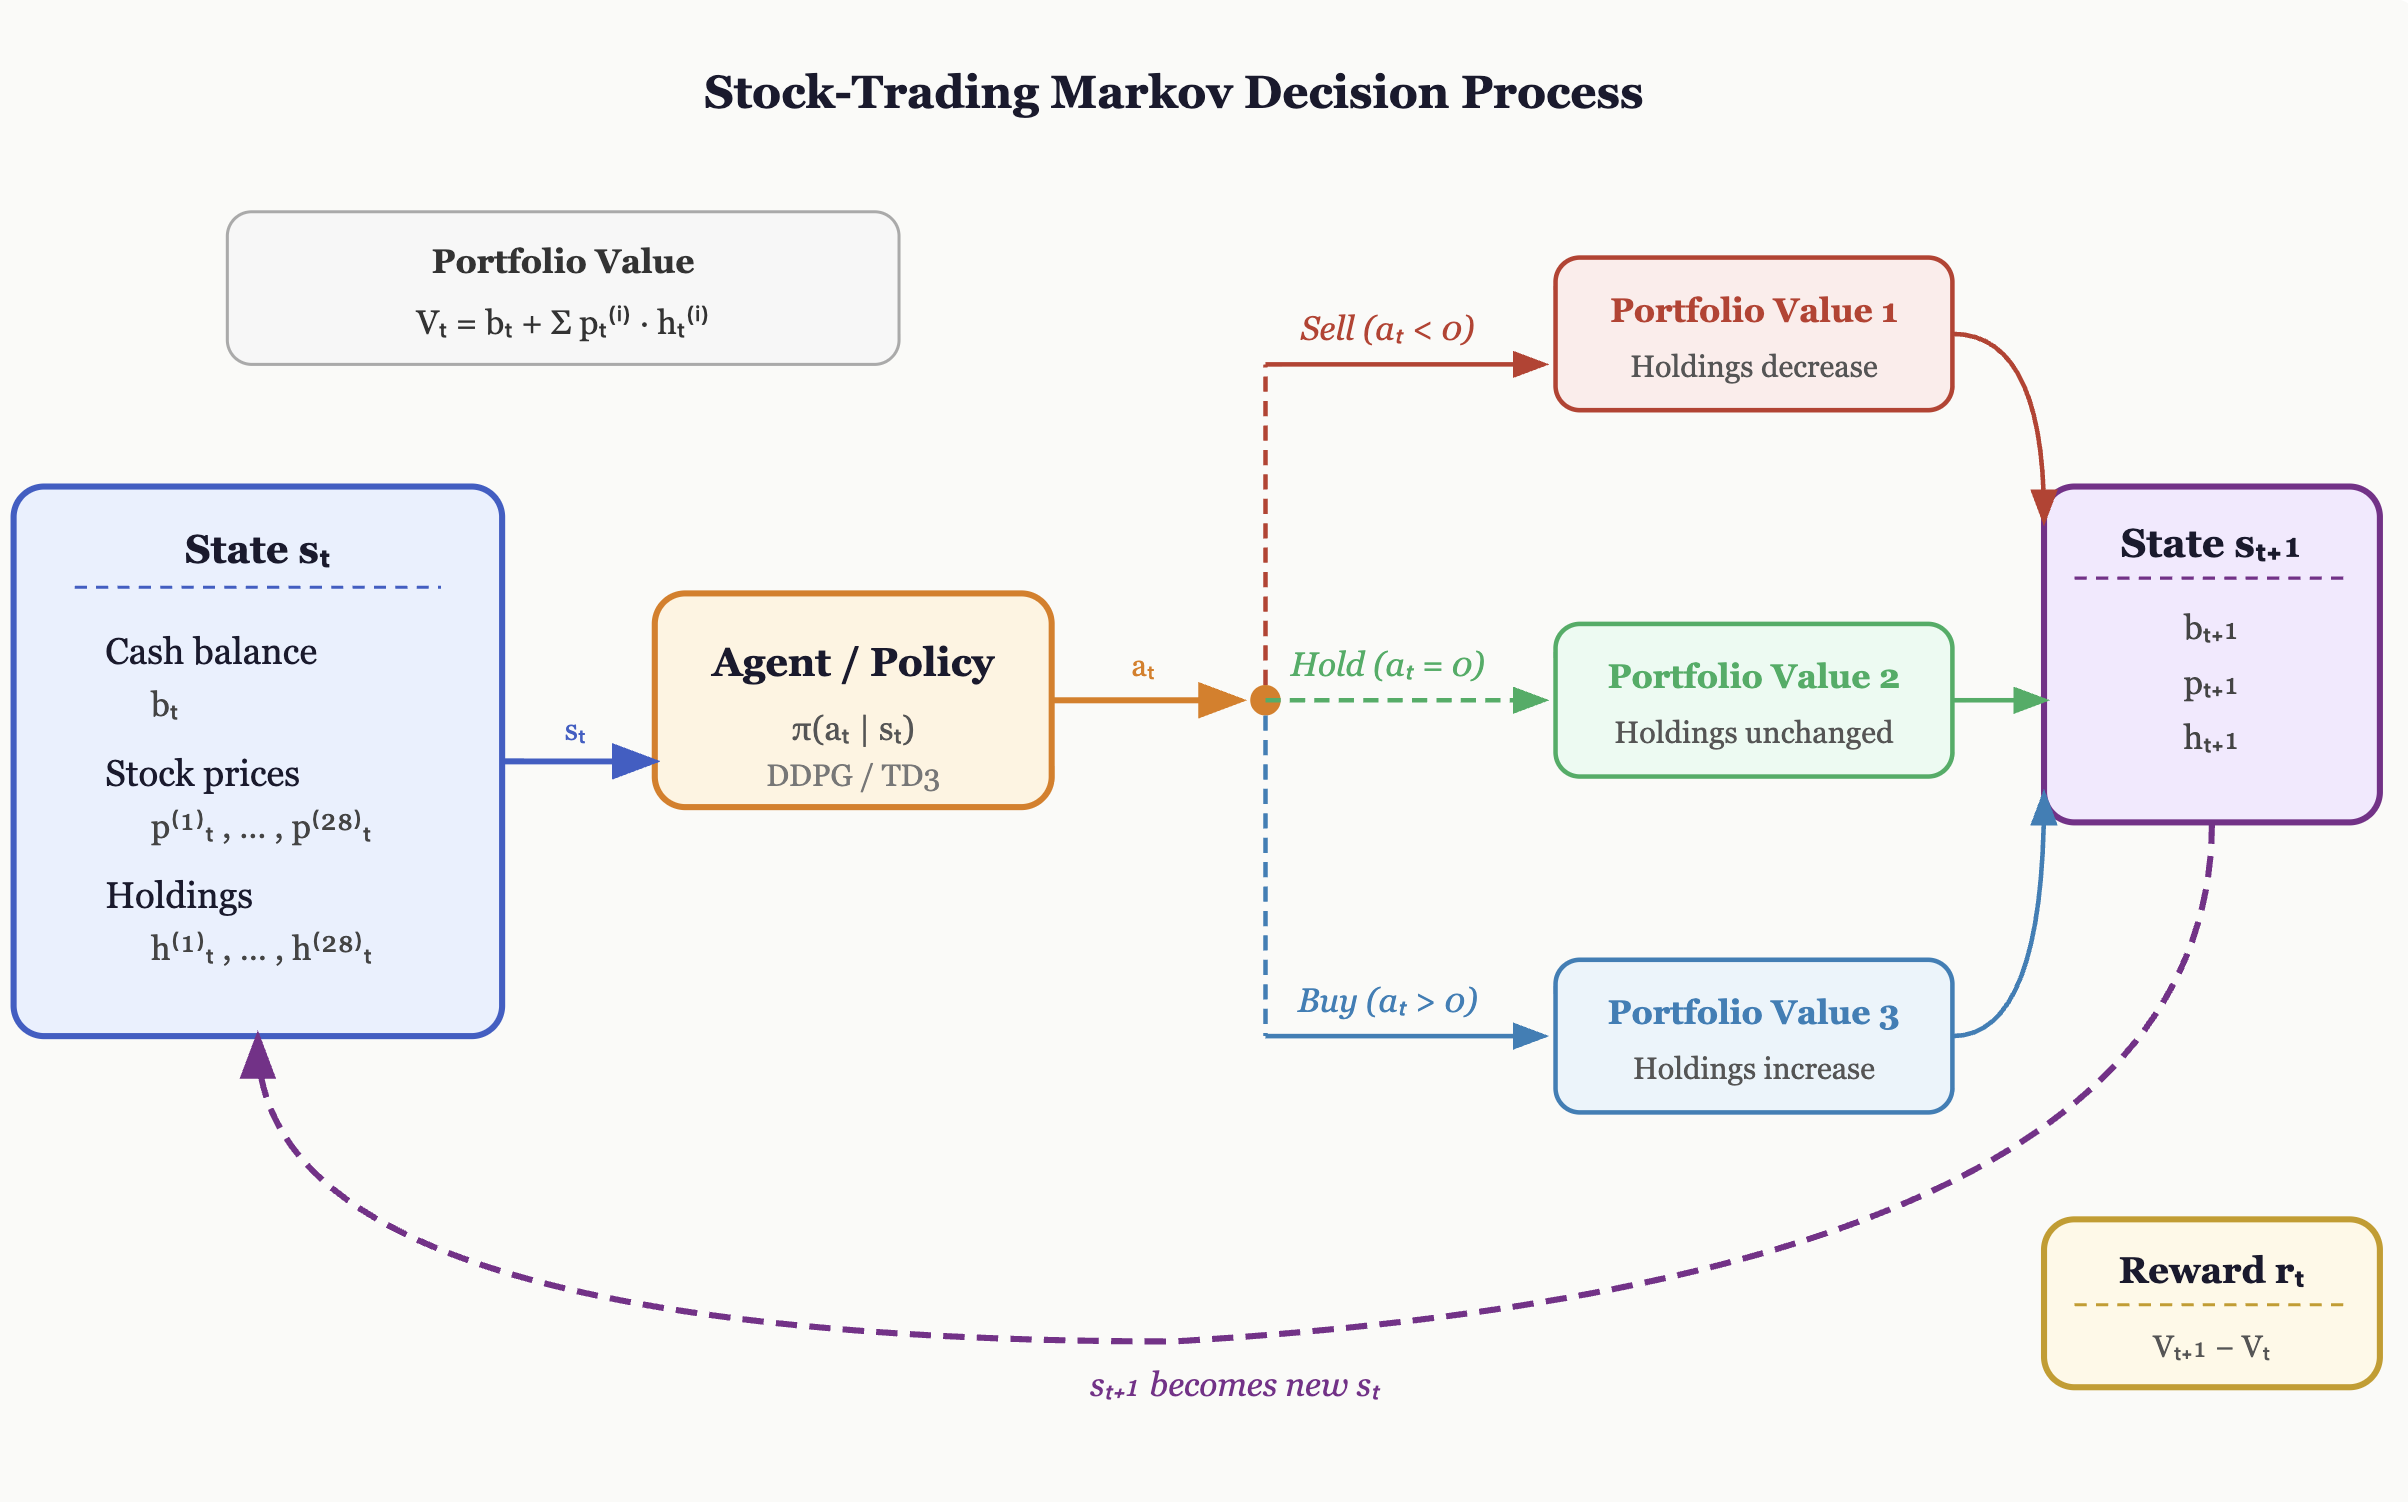
\includegraphics[width=\linewidth,height=0.78\textheight,keepaspectratio]{resources/markov.png}
\end{frame}

\begin{frame}{3) Methods and Experimental Setup}
  \textbf{Algorithms}
  \begin{itemize}
    \item DDPG (paper baseline): deterministic actor-critic, replay buffer, target networks.
    \item TD3: twin critics + delayed actor updates + target smoothing.
  \end{itemize}

  \vspace{0.5em}
  \textbf{Training and evaluation protocol}
  \begin{itemize}
    \item Stable-Baselines3 implementation.
    \item Gymnasium for defining the custom stock trading environment
    \item Data split: train (2009--2014), validation (2015), test (2016--2018).
    \item Hyperparameter tuning with Optuna: 10 trials per algorithm.
    \item Final evaluation: 30 episodes, 3 seeds (42, 43, 44).
  \end{itemize}

  \vspace{0.5em}
  % \textit{Speaker timing: ~40 seconds}
\end{frame}

\begin{frame}{4) Main Results (Test Period 2016--2018)}
  \small
  \begin{tabular}{lcccc}
    \toprule
    Metric & DDPG & TD3 & Min-Var & DJIA \\
    \midrule
    Final Portfolio Value & \$16,141 & \$16,919 & \$13,194 & \$15,595 \\
    Annualized Return & 19.25\% & 21.31\% & 10.74\% & 17.76\% \\
    Annualized Std. & 12.78\% & 12.67\% & 9.37\% & 11.74\% \\
    Sharpe Ratio & 1.51 & 1.68 & 1.15 & 1.51 \\
    \bottomrule
  \end{tabular}

  \vspace{0.75em}
  \begin{itemize}
    \item DJIA is a core benchmark in the original work and in our reproduction.
    \item DDPG slightly beats DJIA on return, with similar Sharpe.
    \item TD3 achieves the strongest overall risk-adjusted performance.
    \item TD3 performs better on average, but with standard deviation considered, it remains close to DDPG.
  \end{itemize}

  % \textit{Speaker timing: ~55 seconds}
\end{frame}

\begin{frame}{Sample Trade Run (DDPG, Seed 42)}
  \centering
  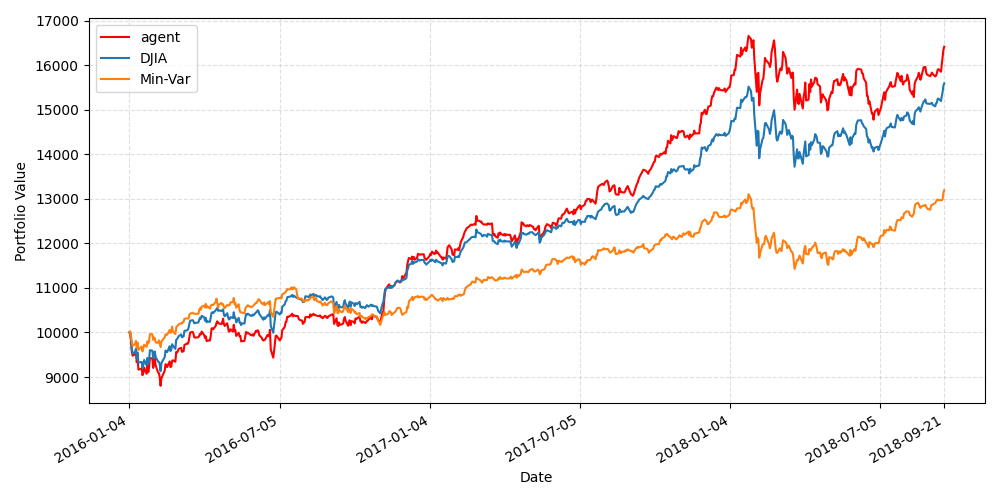
\includegraphics[width=\linewidth,height=0.78\textheight,keepaspectratio]{resources/ddpg_model_test_s42.png}
\end{frame}

\begin{frame}{5) COVID-19 Stress Test (Robustness Check)}
  \small
  \textbf{Setup:} Train on 2010--2019, trade on volatile 2020 (COVID), same Dow Jones universe, best reproduced hyperparameters, 500 episodes, 3 seeds.

  \vspace{0.4em}
  \begin{tabular}{lcccc}
    \toprule
    Metric & DDPG & TD3 & Min-Var & DJIA \\
    \midrule
    Final Portfolio Value & \$10,590 & \$9,786 & \$10,477 & \$10,534 \\
    Annualized Return & 5.93\% & -2.15\% & 4.79\% & 5.36\% \\
    Sharpe Ratio & 0.18 & -0.04 & 0.20 & 0.15 \\
    \bottomrule
  \end{tabular}

  \vspace{0.5em}
  \begin{itemize}
    \item RL does not consistently outperform DJIA and min-variance in this volatile regime.
    \item This questions the original claim that DDPG outperforms classical baselines, since performance degrades under volatile market conditions.
  \end{itemize}
\end{frame}

\begin{frame}{6) Interpretation, Limits, and Future Work}
  \textbf{What we reproduced}
  \begin{itemize}
    \item RL agents outperform min-variance baseline in this setting.
  \end{itemize}

  \textbf{What differed from original paper}
  \begin{itemize}
    \item Reproduced DDPG score is below the reported original DDPG result.
    \item Likely causes: smaller compute budget and less extensive tuning.
  \end{itemize}

  \textbf{Next steps}
  \begin{itemize}
    \item Add transaction costs and slippage.
    \item Increase training/tuning budget and test additional market periods.
    \item Compare against newer methods (e.g., SAC).
  \end{itemize}

  % \textit{Speaker timing: ~45 seconds}
\end{frame}

\begin{frame}{7) Takeaways}
  \begin{itemize}
    \item The original DDPG stock-trading trend is \textbf{partially reproduced}.
    \item \textbf{TD3 outperforms DDPG on the original split}, but not robustly across all regimes.
    \item Reinforcement learning can be promising for portfolio control, but
      realistic assumptions and robust evaluation are critical.
  \end{itemize}

  \vspace{1em}
  \centering
  \Large Thank you.

  \vspace{0.5em}
  \normalsize
  % \textit{Speaker timing: ~25 seconds}
\end{frame}

% \begin{frame}{Backup: 4-Minute Delivery Plan}
%   \begin{itemize}
%     \item Slide 1: 0:00--0:35
%     \item Slide 2: 0:35--1:15
%     \item Slide 3: 1:15--1:55
%     \item Slide 4: 1:55--2:50
%     \item Slide 5: 2:50--3:35
%     \item Slide 6: 3:35--4:00
%   \end{itemize}
% \end{frame}

\end{document}
